% !TeX spellcheck = de_DE
%%%%%%%%%%%%%%
%  COSTANTI  %
%%%%%%%%%%%%%%
%COMANDI DA UTILIZZARE PER TUTTI I DOCUMENTI
% In questa prima parte vanno definite le 'costanti' utilizzate da due o più documenti.

%COMANDI TABELLE
\newcommand{\rowcolorhead}{\rowcolor[HTML]{00ACC1}} %intestazione 
\newcommand{\rowcolorlight}{\rowcolor[HTML]{E0f7fa}} %righe chiare/dispari
\newcommand{\rowcolordark}{\rowcolor[HTML]{80DEEA}} %righe scure/pari
\newcommand{\colorhead}{\color[HTML]{FFFFFF}} %testo intestazione
\newcommand{\colorbody}{\color[HTML]{000000}} %testo righe


%%%%%%%%%%%%%%
%  FUNZIONI  %
%%%%%%%%%%%%%%

% Serve a dare la giusta formattazione al codice inline
\newcommand{\code}[1]{\flextt{\texttt{#1}}}

% Genera automaticamente la pagina di copertina
\newcommand{\makeFrontPage}{
  % Declare new geometry for the title page only.
  \newgeometry{top=4cm}
  
  \begin{titlepage}
  \begin{center}

\begin{center}
  \centerline{
\includegraphics[scale=0.24]{StyleLatex/logo_home.png}}
\end{center}
  
  \vspace{1cm}

  \begin{Huge}
  \textbf{\DocTitolo{}} \\
  \end{Huge}

  \vspace{9pt}  
  
  \begin{tabular}{l|l}
  	\textbf{Nome Gruppo} & WalkAndBuy \\
  	\textbf{Componenti} & Canovese Marco 1094135\\
  	& Zanellato Federico 1094134\\

  \end{tabular}

  \vspace{30pt}
  

  \end{center}
  \end{titlepage}
  
  % Ends the declared geometry for the titlepage
  \restoregeometry
}
%\documentclass[a4paper, oneside, openany]{book}
\documentclass[10pt,a4paper]{extarticle}

%**************************************************************
% Importazione package
%************************************************************** 
\usepackage{graphbox}
% permette di modificare i margini
%\usepackage[top=3.1cm, bottom=3.1cm, left=2.2cm, right=2.2cm]{geometry}
%\usepackage[a4paper]{../../common/style/geometry} %TODO
\usepackage[a4paper, top=2cm, bottom=2.8cm]{geometry}
\usepackage{booktabs} %lista item nelle tabelle
% specifica con quale codifica bisogna leggere i file
\usepackage[utf8]{inputenc}

%indice con i puntini
\usepackage{tocloft}
\renewcommand\cftsecleader{\cftdotfill{\cftdotsep}}



% necessario per risolvere il problema del carattere invisibile per l'a capo
\DeclareUnicodeCharacter{00A0}{ } %?

% per scrivere in italiano e in inglese;
% l'ultima lingua (l'italiano) risulta predefinita
\usepackage[english, italian]{babel}

% imposta lo stile italiano per i paragrafi
\usepackage{parskip}

% fornice elenchi numerati in ordine inverso
\usepackage{etaremune}

\usepackage{caption}

% comandi per l'appendice
\usepackage{appendix}
%\renewcommand\appendixtocname{Appendici} %We really need it?

% import euro symbol
\usepackage{eurosym}

% numera anche i sottoparagrafi
\setcounter{secnumdepth}{5}

% elenca anche i sottoparagrafi nell'indice
\setcounter{tocdepth}{5}

% permetti di definire dei colori
\usepackage[usenames,dvipsnames]{color}

% permette di usare il comando "paragraph" come subsubsubsection!
\usepackage{titlesec}

% permette di inserire le immagini/tabelle esattamente dove viene usato il
% comando \begin{figure}[H] ... \end{figure}
% evitando che venga spostato in automatico
\usepackage{float}

% permette l'inserimento di url e di altri tipi di collegamento
\usepackage[colorlinks=true]{hyperref}

\hypersetup{
    colorlinks=true, % false: boxed links; true: colored links
    citecolor=black,
    filecolor=black,
    linkcolor=black, % color of internal links
    urlcolor=Maroon  % color of external links
}

% permette al comando \url{...} di andare a capo a metà di un link
\usepackage{breakurl}

% immagini
\usepackage{graphicx}

% permette di riferirsi all'ultima pagina con \pageref{LastPage}
\usepackage{lastpage}

% tabelle su più pagine
\usepackage{longtable}

% per avere dei comandi in più da poter usare sulle tabelle
\usepackage{booktabs}

% tabelle con il campo X per riempire lo spazio rimanente sulla riga
%\usepackage{tabularx}

% TABELLE 
% tabelle su più pagine
\usepackage{longtable}

% per avere dei comandi in più da poter usare sulle tabelle
\usepackage{booktabs}

% multirow per tabelle
\usepackage{multirow}

% definisci un nuovo tipo di colonna C che permette di andare a capo con \newline
% e centrata
\usepackage{array}
\usepackage{ragged2e}
%\newcolumntype{P}[1]{>{\RaggedRight\hspace{0pt}}p{#1}}
\newcolumntype{C}[1]{>{\centering\let\newline\\\arraybackslash\hspace{0pt}}m{#1}}

% colore di sfondo per le celle
\usepackage[usenames,dvipsnames,svgnames,table]{xcolor}

% tabelle con il campo X per riempire lo spazio rimanente sulla riga
\usepackage{tabularx}


% personalizza l'intestazione e piè di pagina
\usepackage{fancyhdr}

% permette di inserire caratteri speciali
\usepackage{textcomp}

% permette di aggiustare i margini e centrare tabelle e figure
\usepackage{changepage}

%Permette di includere i grafici a barre
%IMPORTANTE: deve essere caricato prima di /pgfgantt altrimenti causa conflitto
%\usepackage{pgfplots}

% permette di includere i diagrammi Gantt
% su Ubuntu non si può installare il pacchetto, deve essere in modello/
%\usepackage{../../modello/pgfgantt}

% permette di includere i grafici a torta
%\usepackage{../../modello/pgf-pie}

% necessario per pgf-pie
\usepackage{tikz}

% permette i path delle immagini con gli spazi
\usepackage{grffile}

% ruota le immagini
\usepackage{rotating}

% permetti di calcolare le larghezze facendo calcoli
\usepackage{calc}


\fancypagestyle{plain}{
	% cancella tutti i campi di intestazione e piè di pagina
	\fancyhf{}

	\lfoot{
		\DocTitolo{} \ - \textit{\DocRedazione{} \ -  \DocAnno{}}
	}
	\rfoot{Pagina \thepage{} di \pageref{LastPage}}

	% Visualizza una linea orizzontale in cima e in fondo alla pagina
	\renewcommand{\headrulewidth}{0pt}	
	\renewcommand{\footrulewidth}{0.3pt}
}
\pagestyle{plain}

% allarga l'header a tutta la pagina
%\fancyhfoffset[L]{\oddsidemargin + \hoffset + 1in}
%\fancyhfoffset[R]{\evensidemargin + \marginparwidth - \marginparsep}

% Per inserire del codice sorgente formattato

\usepackage{listings}

\lstset{
  extendedchars=true,          % lets you use non-ASCII characters
  inputencoding=utf8,   % converte i caratteri utf8 in latin1, richiede 
  %\usepackage{listingsutf8} anzichè listings
  basicstyle=\ttfamily,        % the size of the fonts that are used for the 
  %code
  breakatwhitespace=false,     % sets if automatic breaks should only happen at 
  %whitespace
  breaklines=true,             % sets automatic line breaking
  captionpos=t,                % sets the caption-position to top
  commentstyle=\color{mygreen},   % comment style
  frame=none,               % adds a frame around the code
  keepspaces=true,            % keeps spaces in text, useful for keeping 
  %indentation of code (possibly needs columns=flexible)
  keywordstyle=\bfseries,     % keyword style
  numbers=none,               % where to put the line-numbers; possible values 
  %are (none, left, right)
  numbersep=5pt,              % how far the line-numbers are from the code
  numberstyle=\color{mygray}, % the style that is used for the line-numbers
  rulecolor=\color{black},    % if not set, the frame-color may be changed on 
  %line-breaks within not-black text (e.g. comments (green here))
  showspaces=false,           % show spaces everywhere adding particular 
  %underscores; it overrides 'showstringspaces'
  showstringspaces=false,     % underline spaces within strings only
  showtabs=false,             % show tabs within strings adding particular 
  %underscores
  stepnumber=5,               % the step between two line-numbers. If it's 1, 
  %each line will be numbered
  stringstyle=\color{red},    % string literal style
  tabsize=4,                  % sets default tabsize
  firstnumber=1      % visualizza i numeri dalla prima linea
}

% Permetti di utilizzare il grassetto per i caratteri Typewriter (per es. il 
%font di \code{...} e \file{...})
\usepackage[T1]{fontenc}
\usepackage{lmodern}


%package added
\usepackage{amsmath}

\usepackage{amsfonts}

%%%%%%%%%%%%%%
%  COSTANTI  %
%%%%%%%%%%%%%%

% In questa prima parte vanno definite le 'costanti' utilizzate soltanto da questo documento.
% Devono iniziare con una lettera maiuscola per distinguersi dalle funzioni.

\newcommand{\DocTitolo}{Relazione progetto TecWeb}

\newcommand{\DocRedazione}{WineNot}

\newcommand{\DocAnno}{Anno 2017/2018}

\title{\textbf{Errori HTML rilevati nel progetto}}
\author{WalkAndBuy}

\date{14 Novembre 2018}

\begin{document}

%\maketitle

\makeFrontPage

\tableofcontents

\newpage

\section{Introduzione}
Il seguente documento intende prendere in analisi gli errori rilevati dal gruppo \textit{Walk and Buy} nel progetto didattico di Tecnologie Web.\\
Quest'analisi si concentra prevalentemente sul codice HTML che risulta essere la parte con la maggior concentrazione di errori.
\\
E’ da tenere presente che la parte \textit{<head>} analizzata nella Home è la medesima in tutte le pagine del sito in quanto è frutto dell’incorporazione del file head.php.\\
Per convenzione \textbf{L\#} è utilizzato se necessario per indicare la riga ove è presente l’errore.

\section{Homepage}

	Gli errori riscontrati nella homepage sono i seguenti:
	\begin{figure}[H]
		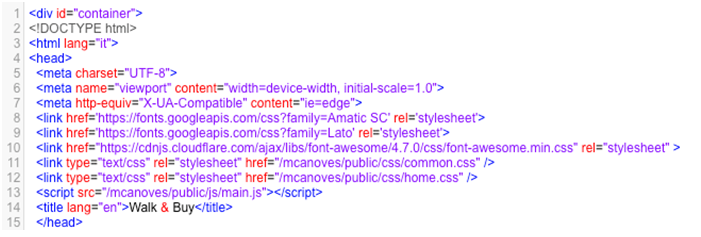
\includegraphics[width=\linewidth]{res/img/home}
		\caption{Codice in testa alla home}
		\label{Codice in testa alla home}
	\end{figure}
	\begin{itemize}
		\item In \textbf{L1}, precedentemente alla dichiarazione DTD \textit{<!DOCTYPE html>} è presente l’apertura di un elemento \textit{<div>} che precede anche la dichiarazione del documento HTML che avviene in \textbf{L3}.\\
		L’errore è risolvibile collocando l’apertura del \textit{<div>} in una posizione più consona a seguito dell’inizio del documento HTML;
		\item In \textbf{L8} è presente un \textit{<link>} di riferimento a un font Google, l’attributo href però contiene una URL con spazio tra \textit{amatic} e \textit{SC}.\\
		Tale dichiarazione è contraria alle norme dello standard che non prevedono la presenza di spazi;
		\item in \textbf{L12} si fa riferimento ad un foglio di stile home.css che non esiste;
		\item Tra \textbf{L19} e \textbf{L48} sono dichiarati alcuni \textit{<div>} che compongo il menù utente e il menù categorie, l’utilizzo di questi div risulta però errato in quanto alcuni di essi risultano aperti ma non chiusi nell’ordine corretto.\\
		Anche in questo caso per porre correzione sarebbe sufficiente riordinare l’ordine di apertura/chiusura dei \textit{<div>} e inserire una chiusura ove necessario al fine di garantire le corrette dipendenze. 
		
	\end{itemize}
\newpage
\begin{figure}[H]
	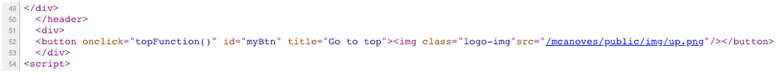
\includegraphics[width=\linewidth]{res/img/home2}
	\caption{Pezzo codice HTML in home}
	\label{Pezzo codice HTML in home}
\end{figure}
\begin{itemize}
	\item In \textit{L52} è assente lo spazio tra l’attributo "\textit{class}" e "\textit{src}";
	\item all’interno del \textit{<body>} sono presenti numerose immagini prive di attributo "\textit{alt}" il quale compromette l’accessibilità del sito web, in particolare risultano sprovviste dell’attributo le icone del menù categorie rendendo quindi inutilizzabile lo stesso da parte di screen reader;
	\item l’\textbf{ID} css "\textit{myImg}" è utilizzato tre volte all’interno del medesimo documento, l’\textbf{ID} è concepito per un utilizzo univoco andrebbero definiti quindi tre ID differenti o in alternativa una \textbf{classe} all’interno del foglio di stile; in quanto risulta essere “legale” solamente la prima dichiarazione di “\textit{myImg}” all’interno del documento.
\end{itemize}
\begin{figure}[H]
	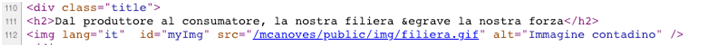
\includegraphics[width=\linewidth]{res/img/home3}
	\caption{Pezzo codice HTML in home}
	\label{Pezzo codice HTML in home}
\end{figure}
\begin{itemize}
	\item In \textbf{L111} è dichiarato un carattere speciale 	"\textit{\&egrave}" privo di punto e virgola terminale, la corretta dichiarazione è "\textit{\&egrave;}" ;
	\item in caso di stampa della pagina non risultano visibili le voci del menù categorie, in quanto il font è di colore bianco. 
\end{itemize}
\section{Pagina Registrazione Utente}
\begin{figure}[H]
	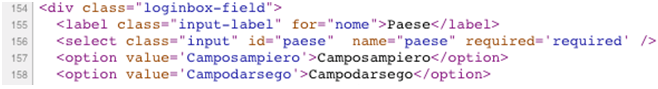
\includegraphics[width=\linewidth]{res/img/regut}
	\caption{Pezzo codice HTML in registrazione utente}
	\label{Pezzo codice HTML in registrazione utente}
\end{figure}
\begin{itemize}
	\item In \textbf{L156} è presente una \textit{<select>} che contiene più elementi figli, vi è un errore in quanto la \textit{<select>}  viene chiusa nella medesima linea senza includere correttamente gli elementi \textit{<option>}. \\ 
	Nella medesima \textit{<select>} inoltre non è presente l’attributo "\textit{size}" per specificare quante voci per volta mostrare nella tendina di selezione. Sarebbe opportuno inserire anche un elemento "\textit{placeholder}";
	\item Il tag \textit{<body>} viene chiuso prematuramente malgrado siano ancora aperti degli elementi figli.
\end{itemize}
\section{Pagina Categoria}
\begin{itemize}
	\item Oltre agli errori riferiti alla parte \textit{<head>}.
	I pulsanti per aggiungere al carrello gli articoli in vetrina non sono corredati dell’attributo "\textit{alt}" risultano per cui inaccessibili e inutilizzabili da utenti che fanno ricorso a screen reader, medesime considerazioni valgono per il pulsante "\textit{scoprili tutti}";
	
	\item Stampando la pagina risulta completamente alterata la disposizione dei prodotti in vetrina, in particolare alcuni prodotti spariscono e non vengono stampati a causa della mancanza di un foglio di stile dedicato. 
\end{itemize}
\section{Pagina Singolo Prodotto}
\begin{itemize}
	\item In questa pagina è presente un carattere speciale dichiarato privo di punto e virgola.
	Nell’elemento \textit{<button>} ovvero il pulsante per aggiungere al carrello è presente l’attributo "\textit{alt}" anziché l’attributo "\textit{title}" previsto per i button;
	
	\item \textbf{L142} è presente un elemento \textit{<h4>} chiuso erroneamente con un tag privo di /.  
\end{itemize}
\section{Pannello Amministrativo}
\begin{itemize}
	\item E’ presente l’attributo "\textit{type = ‘select’}" all’interno dell’elemento \textit{select,} il quale non è necessario. Ed è chiuso il tag \textit{<select>} nella medesima riga di apertura senza includere gli elementi figli \textit{<option>};
	
	\item Come rilevato nella pagina di registrazione anche in questa non è presente un attributo "\textit{size}" ed un "\textit{placeholder}" nella \textit{<select>}.   
\end{itemize}

\section{Inserimento Nuovo Articolo}
\begin{itemize}
	\item Nel form di inserimento ordine, si rilevano i medesimi errori riscontrati nelle altre pagine per quanto riguarda le \textit{<select>};
	
	\item \textit{<form>} viene chiuso prima della chiusura di tutti gli elementi figli contenuti in esso, in questo caso è presente un \textit{<div>} interno;   
	
	\item lato php mancano accurati controlli sui dati inseriti nei vari campi.
\end{itemize}
\end{document}